\documentclass[handout]{beamer}
%\documentclass [serif,mathserif,professionalfont]{beamer} 
%\usepackage {pxfonts}
%\usepackage {eulervm}
%\usepackage{mathpazo}
%\logo{\includegraphics[height=1.2cm]{fsulogo.png}}

\usepackage{tikz}
\usepackage{graphicx}
\usepackage{multimedia}
\usepackage{booktabs}
\usepackage{multirow}
\usepackage{amssymb}
\usepackage{amsmath}
\usepackage[latin1]{inputenc}
%\usetheme{Warsaw}
\usecolortheme{lily}
\setbeamercovered{transparent}
%\useoutertheme[subsection=false]{smoothbars}

\title[EVA, Ann Arbor, MI 2015 \insertdate]{Weakly-supervised Learning in Computer Vision and Medical Imaging}

\author{Fengbei Liu}
\institute{Australian Institute for Machine Learning (AIML) \\University of Adelaide, Australia}
\date{Oct 17, 2023}

\begin{document}

\begin{frame}
\titlepage
% \tiny Supervisor: Prof. Gustavo Carneiro, Prof. Mark Jenkinson
\end{frame}

\section{}

\begin{frame}{Supervised learning}
% \begin{center}
% {\Large Supervised learning}\\
% \vspace{.5cm}
\begin{itemize}
    \item Achieves great success, surpassing human-level error rate on ImageNet classification 2017.\footnote[1]{\tiny Olga Russakovsky et al. Imagenet large scale visual recognition challenge. IJCV 2015}
    \item SENet Top 5 error rate 2.43\%, human Top 5 error rate 5.1\%
    \item Requires \underline{large amount} of \underline{accurate} ground truth labels.
\end{itemize}
% \includegraphics[scale = .25]{figures/TornMeso2.jpg}
% \end{center}
\end{frame}

\begin{frame}{Weakly-supervised learning}
Weakly-supervised learning aims to learn from imperfect scenario\footnote[2]{\tiny Zhi-Hua Zhou. A brief introduction to weakly supervised learning. National
science review, 2018}:
\begin{itemize}
\item Incomplete supervision \\
Only a subset of samples labeled and large amount of unlabeled samples.
\item Inaccurate supervision \\
Ground truth labels contain noise.
\item many others ...
\end{itemize}

\end{frame}


\begin{frame}{A simple demo of each scanerio}
\begin{figure}
    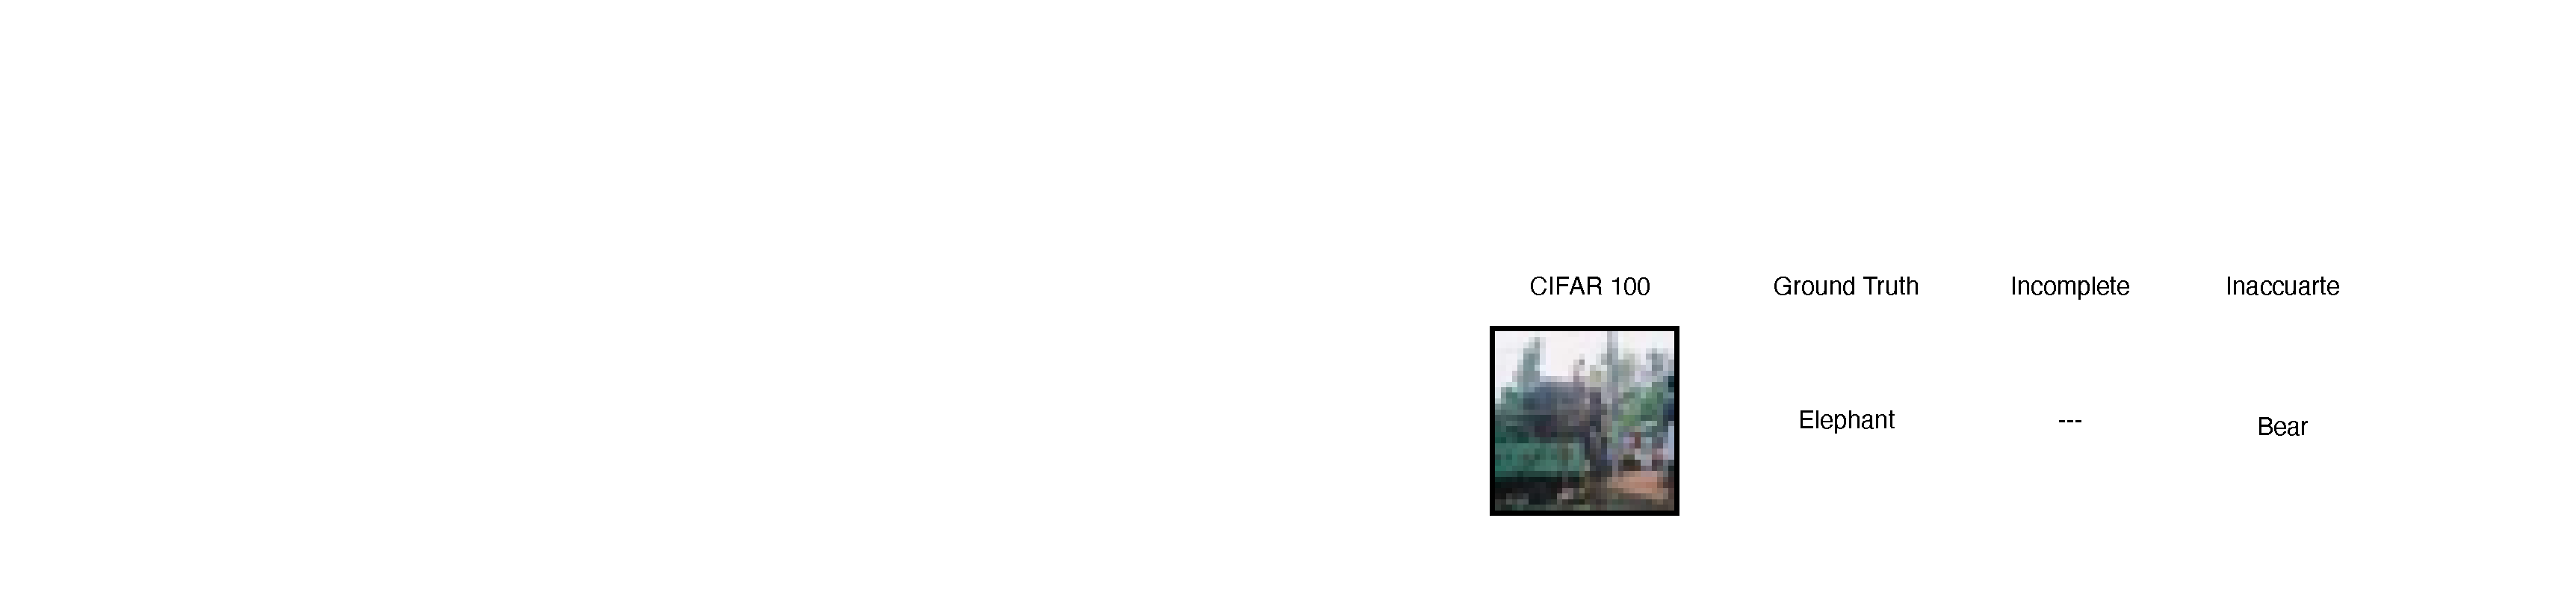
\includegraphics[width=\linewidth]{figures/WL_demo.pdf}
\end{figure}
\end{frame}


\begin{frame}{Datasets: computer vision \& medical imaging analysis (MIA)}
    \begin{itemize}
        \item CV: Multi-class, balance distribution, good pre-train weights (ImageNet)
        \item MIA: Multi-label, extreme imbalanced distribution, domain gap with ImageNet pre-train\footnote[3]{\tiny Raghu, Maithra, et al. "Transfusion: Understanding transfer learning for medical imaging." NeruIPS (2019).}
    \end{itemize}
    This impose challenges, particularly for weakly-supervised methods on MIA datasets.
\end{frame}

\begin{frame}{A quick look at medical datasets we used}
    \begin{figure}
        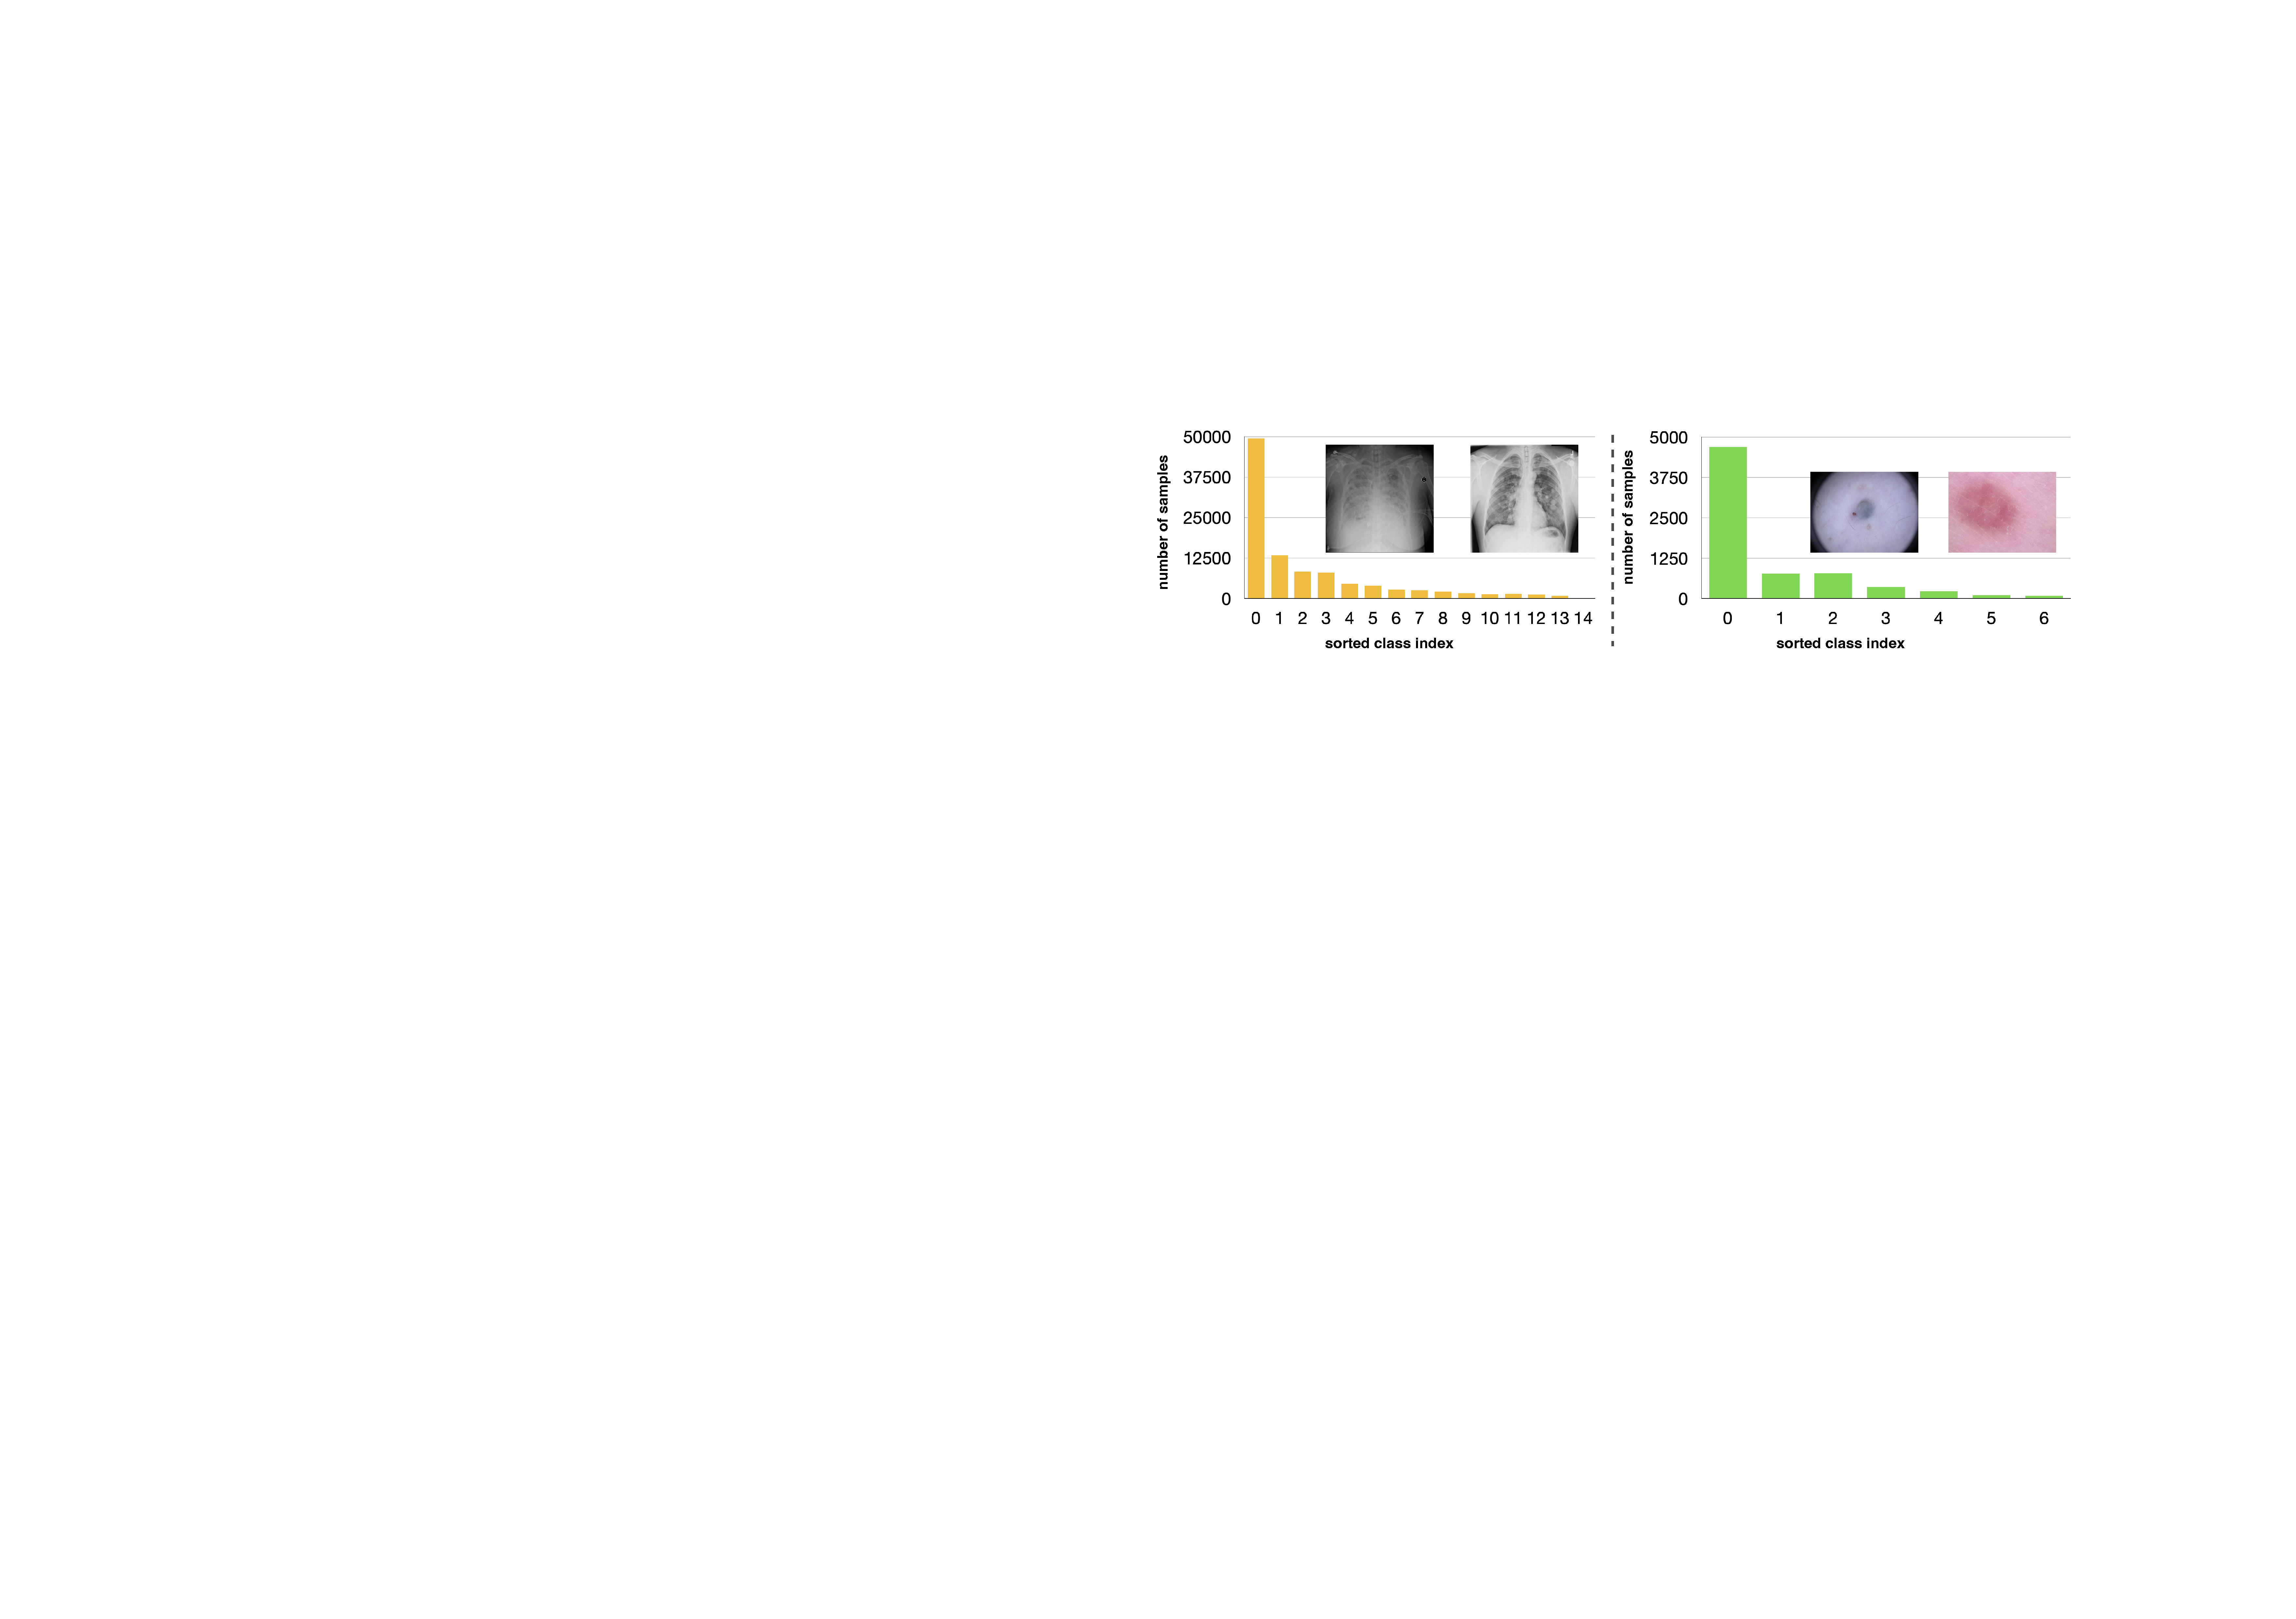
\includegraphics[width=\linewidth]{figures/data_distribution.pdf}
    \end{figure}
    Left is NIH Chest X-ray14 (multi-label), right is ISIC2018 (multi-class)
\end{frame}

\begin{frame}{Incomplete supervision}
    Two typical approaches:
    \begin{itemize}
        \item Semi-supervised Learning (SSL) \\
        No oracle \\
        Learning from all samples (labeled + unlabeled)\\
        aiming for best performance.
        \item Active learning (AL)\\
        With oracle \\
        Learning from selected samples (labeled + most informative unlabeled samples ) \\
        aiming for best performance, under a fixed budget.
    \end{itemize}
    We will be focusing on \underline{SSL} method.
\end{frame}

\begin{frame}{Self-supervised pre-training}
Self-supervised pre-training is a great way for SSL methods
\begin{itemize}
    \item Agnostic to multi-class/multi-label 
    \item Robust to data imbalance \footnote[4]{\tiny Liu, Hong, et al. "Self-supervised learning is more robust to dataset imbalance". ICLR 2021.}
    \item Meaningful weight for MIA datasets
\end{itemize}
we investigate contrastive learning based self-supervised pre-training on NIH Chest X-ray14, CheXpert and ISIC2018 datasets for SSL setup.
\end{frame}

\begin{frame}{Self-supervised pre-training (Cont.)}
    MIA adaptions:
    \begin{itemize}
        \item Batch size issue \checkmark \\
        Follow MoCo\footnote[5]{\tiny He, Kaiming, et al. "Momentum contrast for unsupervised visual representation learning". CVPR, 2020.}, we used memory bank.
        \item Random cropping may breaks in multi-label \checkmark \\
        Multiple crops to estimate a Gaussian distribution and sample positive from Gaussian \footnote[6]{\tiny Cai, Qi, et al. "Joint contrastive learning with infinite possibilities." NeurIPS 2020}.
        \item Some augmentations are not needed \checkmark \\
        Remove random grayscale, color distortion.
        \item MIA unique augmentations $\times$ \\
        Elastic transformation, histogram equalization. 
        \underbar{No significant improve, and they are too slow}
    \end{itemize}
\end{frame}

\begin{frame}{Self-supervised pre-training (Cont.)}
    \begin{table}[t!]
        \centering
        \scalebox{0.9}{
        \begin{tabular}{c|c|c|c|c|c|c}
        \hline
        Label Percentage  & 2\%           & 5\%            & 10\%           & 15\%           & 20\%  & 100\% \\ \hline
        Graph XNet*         & 53.00            & 58.00             & 63.00            & 68.00             & 78.00    & N/A   \\
        SRC-MT*           & 66.95         & 72.29          & 75.28          & 77.76          & 79.23 & 81.75 \\
        NoTeacher  & 72.60 & 77.04 & 77.61 & N/A &79.49 &N/A\\
        MoCo V2      &    65.97      &    73.84     &    77.07      &    79.37       & 80.17 & 81.20  \\ \hline
        Ours     & \textbf{74.69} & \textbf{78.96} & \textbf{79.90} & \textbf{80.31} & \textbf{81.06}    &   \textbf{82.51} \\\bottomrule
        \end{tabular}
        }
        \caption{Mean AUC result over the 14 disease classes of Chest X-Ray14 for different label set training percentages. * indicates the methods that use Densenet169 as backbone architecture. Rest are Densetnet121. 
        }
        \label{tab:main}
        \end{table}
        \small Liu, Fengbei, et al. "Self-supervised mean teacher for semi-supervised chest x-ray classification." MICCAI-MLMI 2021.
\end{frame}

\begin{frame}{Pseudo-labelling}
    Pseudo-labelling is the earliest method for SSL, works for both multi-class/multi-label\footnote[7]{\tiny Rizve, Mamshad Nayeem, et al. "In defense of pseudo-labeling: An uncertainty-aware pseudo-label selection framework for semi-supervised learning." ICLR 2021}. But:
    \begin{itemize}
        \item Estimating threshold, particularly for each class in multi-label
        \item High-confidence pseudo labels are biased towards data imbalance
    \end{itemize}
    Improving pseudo-labeling method, address these two issues.
\end{frame}

\begin{frame}{High-informative unlabeled samples}
    High-confidence pseudo label vs. High-informative unlabeled samples
    \begin{itemize}
        \item Informativeness: feature similarity between unlabeled and labeled samples \\
        KNN graph, Faiss library
        \item High-informative: unlabeled samples with low feature similarity with labeled samples
        \item Gaussian Mixture Model (GMM) for partitioning, no threshold
        \item Ensemble linear classifier and KNN classifier for supervision
    \end{itemize}
\end{frame}

\begin{frame}{Experiment results}
    \begin{table}[t!]
        \centering
        \caption{Mean AUC testing set results over the 14 disease classes of Chest X-Ray14 for different labelled set training percentages. * indicates the methods that use DenseNet-169 as backbone architecture. \textbf{Bold} number means the best result per label percentage and \underline{underline} shows previous best results. %\fengbei{We run experiments three times and take the highest result. 
        }
        \label{tab:main}
        \scalebox{0.8}{
        \begin{tabular}{c|l|c|c|c|c|c}
        \toprule \hline 
        Method Type & Label Percentage  & 2\%           & 5\%            & 10\%           & 15\%           & 20\%  \\ \hline
        \multirow{3}{*}{Consistency based} & SRC-MT*          & 66.95         & 72.29          & 75.28          & 77.76          & 79.23 \\
                                          & NoTeacher  & 72.60 & 77.04 & 77.61 & N/A &79.49\\ 
                                         & S$^2$MTS$^2$ & \underline{74.69} & \underline{78.96} & \underline{79.90} & \underline{80.31}  &\underline{81.06}   \\ \hline
        \multirow{2}{*}{Pseudo Label} & Graph XNet*         & 53.00            & 58.00             & 63.00            & 68.00             & 78.00     \\
        & UPS &   65.51      & 73.18  &        76.84       &      78.90         &         79.92          \\              
        & Ours     & \textbf{74.82} & \textbf{79.20} & \textbf{80.40} & \textbf{81.06} & \textbf{81.77}     \\ \hline  \bottomrule
        \end{tabular}
        }
        \end{table}   
\end{frame}

\begin{frame}{Distribution visualization}
    \begin{figure}
        \includegraphics[page=6,width=\linewidth]{figures/Full_DD.pdf}
    \end{figure}
    \tiny Liu, Fengbei, et al. "ACPL: Anti-curriculum pseudo-labelling for semi-supervised medical image classification." CVPR 2022.
\end{frame}

\begin{frame}{Inaccurate supervision (noisy label learning)}
    Chest X-ray datasets use NLP tools to extract labels from radiology report, creating noisy labels. \\
    Three typical approaches for NLL:
    \begin{itemize}
        \item Sample selection \\
        Small-loss assumption: model will fit clean samples first (small-loss) and fit noisy samples later (large loss) \\
        Combine with SSL
        \item Robust loss \\
        Mean Absolute Error (MAE) is robust to label noise but hard to train \\
        Combine MAE with CE
        \item Transition matrix \\
        % Guarantee to converge to optimal clean classifier \\
        $p(\tilde{Y}|X) $ = $p_{\theta_1}(\tilde{Y}|Y,X) p_{\theta_2}(Y|X)$ \\
        Requires additional regularization, anchor points
    \end{itemize}
    % we will be focusing on robust loss for MIA and transition matrix for CV
\end{frame}

% \begin{frame}{NLL for MIA}
%     \begin{itemize}
%         \item Sample selection
%         \item \underline{Robust loss is fine.}
%         \item Transition matrix co-occur with multi-label correlation matrix.
%     \end{itemize}

% \end{frame}

\begin{frame}{Robust loss for MIA}
    For noisy label:
    \begin{itemize}
        \item Gradient of CE: $ \nabla \ell_{CE}(\mathcal{S},\theta) =\frac{1}{|\mathcal{S}|}\sum_{i \in \mathcal{S}} \mathbf{J}_{\mathbf{x}^i}(\theta)(\mathbf{p}^i - \mathbf{\tilde{y}}^i)$ \\
        $\mathcal{S}$ is training set, $\mathbf{J}$ is Jacobian matrix, $\mathbf{p}$ is prediction and $\tilde{y}$ is noisy ground truth
        \item Overfit noisy label because no gradient on clean label
        \item \underline{Maintain clean label gradient in later training}
        \item Store a moving average of early prediction logits and regularize training
        \item $\ell_{REG}(\mathbf{t}^i,\mathbf{p}^i) =
        \log(1 - \sigma
        (\mathbf{t}^i)^{\top}\mathbf{p}^i)$
    \end{itemize}
    For data imbalance:
    \begin{itemize}
        \item Logits adjustment\footnote[8]{\tiny Menon, Aditya Krishna, et al. "Long-tail learning via logit adjustment." ICLR 2021.}: adds a label-dependent prior (the empirical class frequencies on training set) to each logits
        \item $\log P(Y|X) - \log P_{train}(Y) + \log P_{test}(Y)$
    \end{itemize}
\end{frame}

\begin{frame}{Framework}
    \begin{figure}
        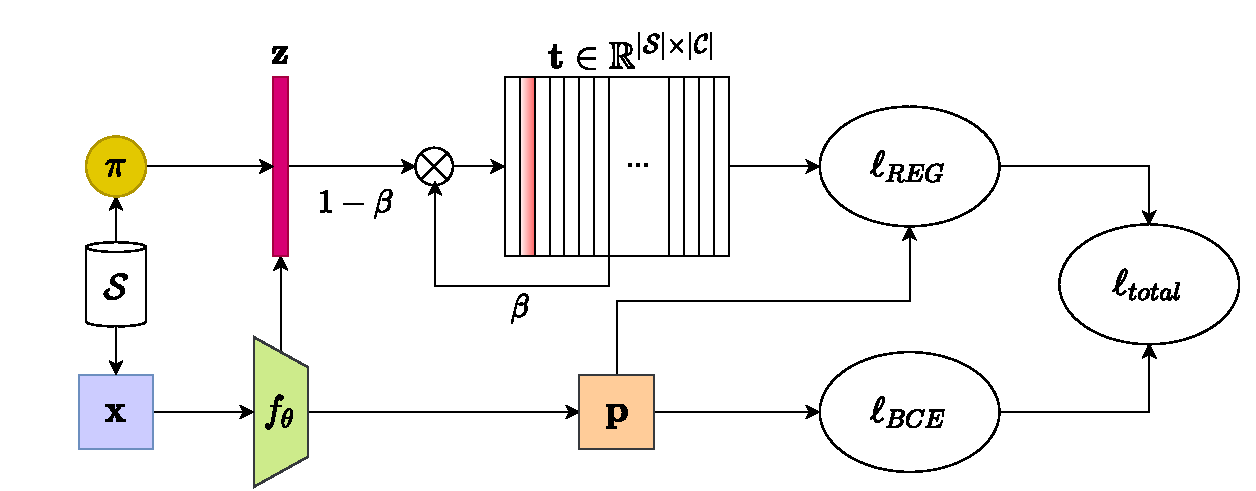
\includegraphics[width=\linewidth]{figures/framework (1).pdf}
    \end{figure}

\end{frame}

\begin{frame}{Experiment results}
   Train on CheXpert (CXP), test on OpenI (OPI) or PadChest (PDC)
   \begin{table}[t]
    \centering
    \caption{Class-level and mean testing AUC on OPI and PDC for the experiment based on training on CXP. Best results for OPI/PDC are in \textbf{bold}/\underline{underlined}.}
    \label{tab:cxp_result}
    \resizebox{0.9\textwidth}{!}{
    \begin{tabular}{l|cc|cc|cc|cc|cc}
    \toprule \hline
    Methods             & \multicolumn{2}{c|}{CheXNet} & \multicolumn{2}{c|}{Hermoza et al. } & \multicolumn{2}{c|}{Ma et al.} & \multicolumn{2}{c|}{DivideMix} & \multicolumn{2}{c}{Ours} \\ \hline
    Datasets     & OPI          & PDC          & OPI             & PDC            & OPI             & PDC             & OPI           & PDC           & OPI         & PDC         \\ \hline
    Cardiomegaly & 84.00           & 80.00           &  87.01               &  87.20              &     82.83            &    85.89             &    71.14           &   66.51            & \textbf{88.86}       & \underline{88.48}       \\
    Edema        & 88.16        & 98.80         &  87.92               &   98.72             &86.46                      &      97.47           &     75.36         &    95.51           & \textbf{88.63}       & \underline{99.60}        \\
    Pneumonia    & \textbf{65.82}        & 58.96        &   65.56              &    53.42            &   61.88              &     54.83            &    57.65           &     40.53          & 64.90        & \underline{67.89}       \\
    Atelectasis  & 77.70         & 72.23        &   78.40              &   \underline{75.33}             &  80.13               &    72.87             &    73.65           &    64.12           & \textbf{80.81}       & 75.03       \\
    Pneumothorax & 77.35        & \underline{84.75}        &   62.09              &    78.65            &  51.08               &     71.57             &     68.75          &      54.05         & \textbf{82.18}       & 83.32       \\
    Effusion     & 85.81        & 91.84        &   87.00              &    \underline{93.44}            &  \textbf{88.43}               &     92.92            &    78.60           &    79.89           & 83.54       & 89.74       \\
    Fracture     & 57.64        & 60.26        &   57.47              &    53.77            &   59.92              &    60.44             &    \textbf{60.35}           &    59.43           & 57.02       & \underline{62.67}       \\ \hline
    Mean AUC     & 76.64        & 78.12        &  75.06               &    77.29            &   72.96              &    76.57             &    69.36           &    65.72           & \textbf{77.99}       & \underline{80.96}   \\ \hline \bottomrule
    \end{tabular}}
    % \caption{Training on CXP~\cite{irvin2019chexpert} and testing on OPI~\cite{demner2016preparing} and PDC~\cite{bustos2020padchest} class-level and mean AUC results.}
    % \label{tab:cxp_result}
    \end{table}
    \tiny Liu, Fengbei, et al. "NVUM: Non-volatile Unbiased Memory for Robust Medical Image Classification." MICCAI 2022.
\end{frame}


\begin{frame}{Transition matrix for CV}
    \begin{itemize}
        \item Generative modeling solves identifiability issue of transition matrix
        \item $p(X,Y,\tilde{Y},Z) = p(Y)p(Z)p(X|Y,Z)p(\tilde{Y}|Y,X)$
        \item Adding constraint on $p(X|Y,Z)$ will encourage identifiability of transition matrix $p(\tilde{Y}|Y,X)$
    \end{itemize}
    However:
    \begin{itemize}
        \item This requires a generative model (VAE,GAN)
        \item The ability for generating images does not help classification task\footnote[9]{\tiny Dai, Zihang, et al. "Good semi-supervised learning that requires a bad gan." NeurIPS 2017.}
        \item $p(Y)$ is usually assume uniform prior
    \end{itemize}
\end{frame}

\begin{frame}{Framework of generative modeling of transition matrix}
    \begin{figure}
        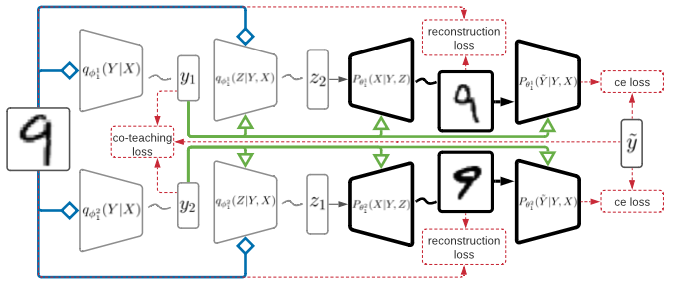
\includegraphics[width=\linewidth]{figures/Screenshot 2023-10-17 at 16.47.05.png}
    \end{figure}
    \tiny Yao, Yu, et al. "Instance-dependent label-noise learning under a structural causal model." NeurIPS 2021.
\end{frame}

\begin{frame}{Transition matrix for CV}
    Remove $Z$:
    \begin{itemize}
        \item $p(X,Y,\tilde{Y}) = p(Y)p(X|Y)p(\tilde{Y}|Y,X)$
        \item $p(X|Y)$ is intractable due to infinite number of $X$ given only $Y$
        \item Approximate it within finite training samples:
        $p(\mathbf{x}|\mathbf{y}) \propto \frac{q(\mathbf{y} | \mathbf{x})}{\sum_{i=1}^{|\mathcal{D}|} q(\mathbf{y} | \mathbf{x}_i)}$ \\
        $q(\mathbf{y} | \mathbf{x})$ is the variational posterior 
    \end{itemize}
    Non-uniform $p(Y)$:
    \begin{itemize}
        \item Inspired by partial label learning decomposition\footnote[10]{\tiny Qiao, Congyu, Ning Xu, and Xin Geng. "Decompositional Generation Process for Instance-Dependent Partial Label Learning." ICLR 2022.}, a non-uniform $p(Y)$ is proposed:
        \item $p_i(\mathbf{y}(j)) = \frac{\tilde{\mathbf{y}}_i(j) + \mathbf{c}_i(j) +  \mathbf{u}_i(j)}{Z}$
        \item $\mathbf{c}_i(j)$ is clean label coverage, $\mathbf{u}_i(j)$ is clean label uncertainty. All in one-hot form.
    \end{itemize}
\end{frame}

\begin{frame}{Our framework}
    Based on previous contribution, we build our framework:
    \begin{itemize}
        \item  $ \log p(\mathbf{x} | \mathbf{y} ) = \log \frac{p(\tilde{\mathbf{y}},\mathbf{y} , \mathbf{x})}{p(\tilde{\mathbf{y}} | \mathbf{x}, \mathbf{y})p(\mathbf{y})}.$
        % \item $\mathbb{E}_{q(\mathbf{y} | \mathbf{x})} \left [\log p(\mathbf{x} | \mathbf{y}) \right ] = \mathbb{E}_{q(\mathbf{y}| \mathbf{x})} \left[ \log p(\tilde{\mathbf{y}}| \mathbf{x} , \mathbf{y})  \right] 
        % %+ \mathbb{E}_{q(\mathbf{y}| \mathbf{x})} \left[ \log  \frac{p(\mathbf{x}|\mathbf{y})p(\mathbf{y})} {q(\mathbf{y} | \mathbf{x})}  \right] 
        % - \mathsf{KL}\left[q(\mathbf{y} | \mathbf{x}) \| p(\mathbf{x}|\mathbf{y})p(\mathbf{y}) \right]
        % + \mathsf{KL}\left[q(\mathbf{y} | \mathbf{x}) \|p(\tilde{\mathbf{y}} | \mathbf{x}, \mathbf{y})p(\mathbf{y}) \right].$
    \end{itemize}
    \begin{figure}
        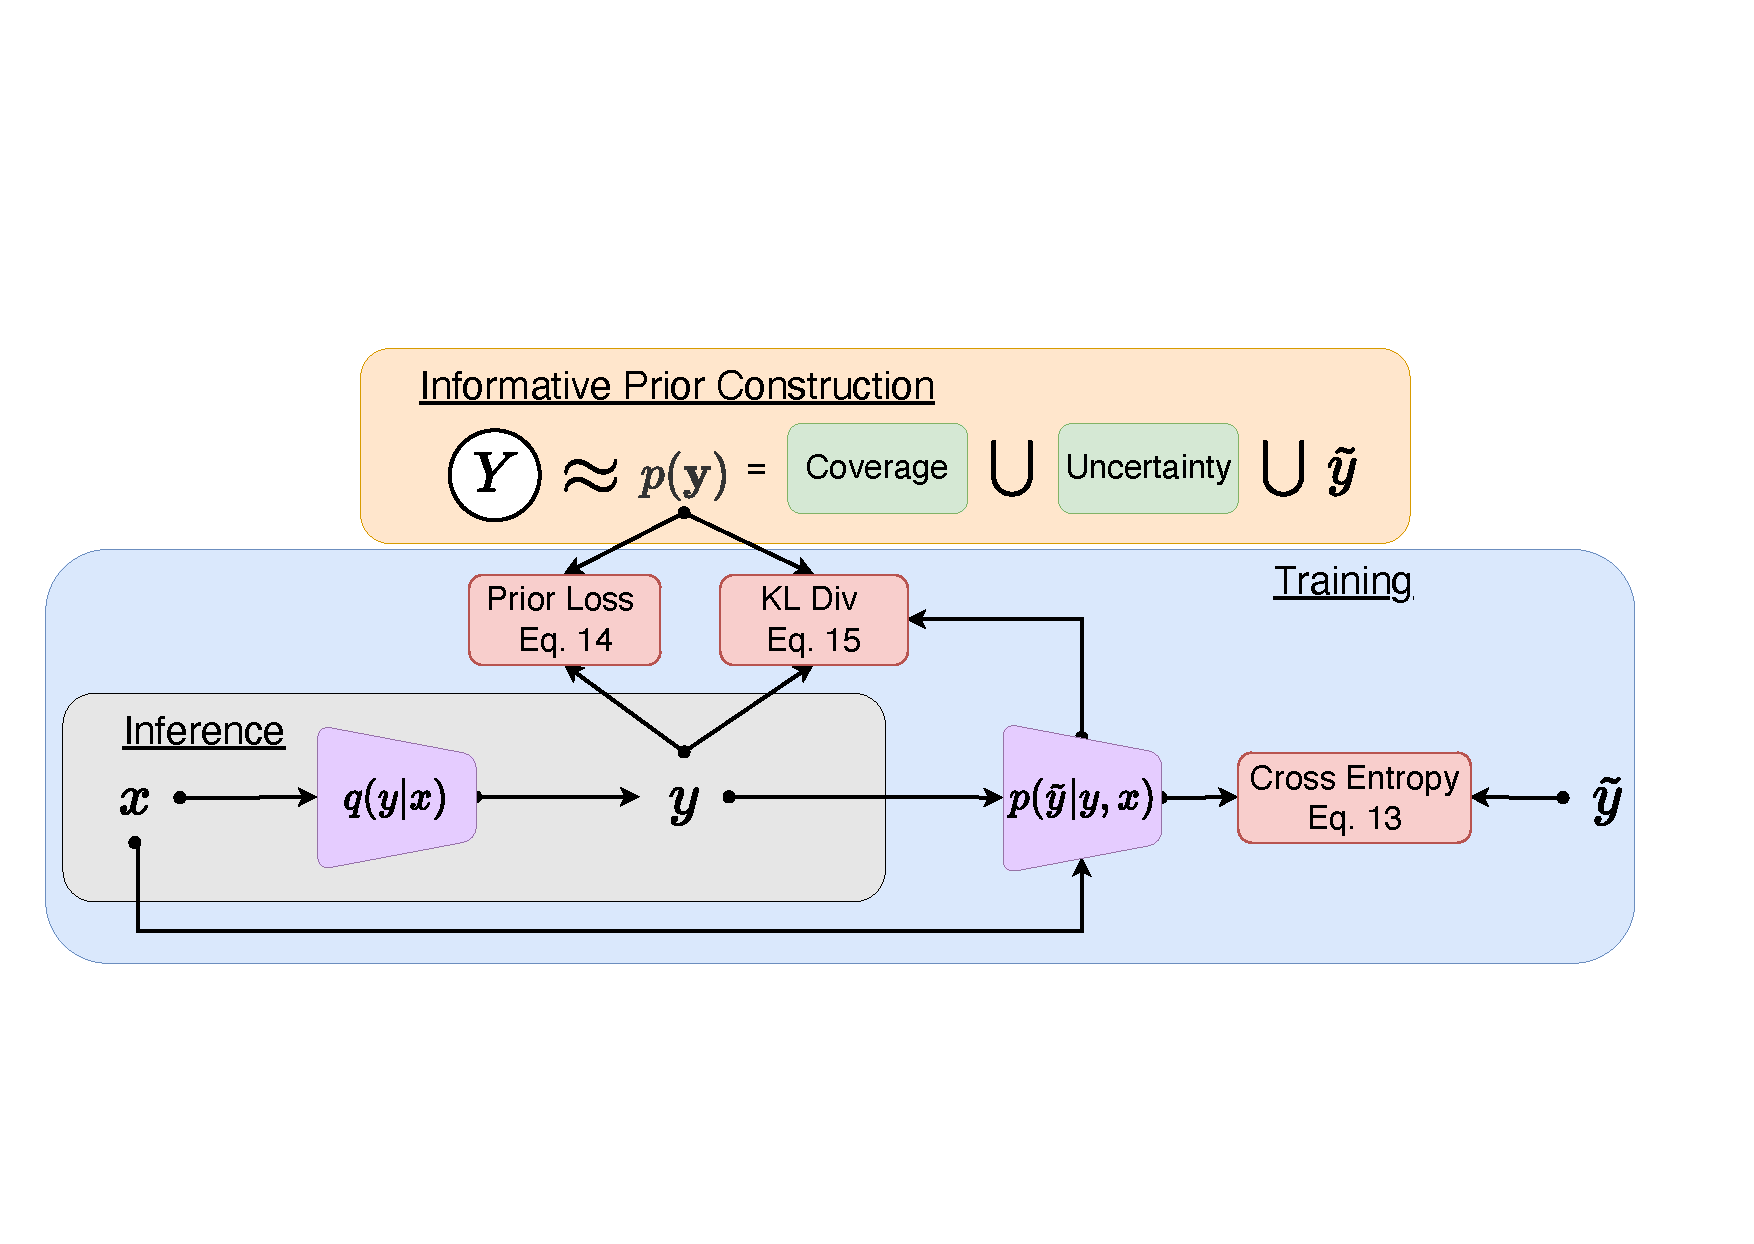
\includegraphics[width=\linewidth]{figures/GNL-Page-1.drawio.pdf}
    \end{figure}
\end{frame}


\begin{frame}{Experiment results}
    We tested under synthetic CV benchmarks, real-world CV datasets, NLP benchmarks 
    \begin{table}[t!]
        \centering
        \scalebox{0.85}{
        \begin{tabular}{l|cccc}
         \toprule \hline 
        \multirow{2}{*}{Method} & \multicolumn{4}{c}{CIFAR100}                                                               \\ \cline{2-5} 
                                & $20\%$           & $30\%$           & $40\%$              & $50\%$    \\ \hline
        CE                      &  63.94$\pm$0.51   & 61.97$\pm$1.16   & 58.70$\pm$0.56   & 56.63$\pm$0.69   \\
        %GCE~\cite{Zhang_NeurIPS_2018_Generalized_CE}                      & 68.35$\pm$0.33   & 66.35$\pm$0.13   & 62.09$\pm$0.09   & 56.68$\pm$0.75   \\
        DMI                     & 64.72$\pm$0.64   & 62.8$\pm$1.46    & 60.24$\pm$0.63   & 56.52$\pm$1.18   \\
        Forward          & 67.23$\pm$0.29   & 65.42$\pm$0.63   & 62.18$\pm$0.26   & 58.61$\pm$0.44   \\
        CoTeaching             & 67.40$\pm$0.44   & 64.13$\pm$0.43   & 59.98$\pm$0.28   & 57.48$\pm$0.74   \\
        % CoTeaching+~\cite{yu2019does}            & 68.30$\pm$0.69   & 65.77$\pm$0.30   & 61.75$\pm$0.53   & 57.94$\pm$0.15   \\
        % JoCor~\cite{wei2020combating}                   &  67.87$\pm$0.80   & 65.73$\pm$0.55   & 61.64$\pm$0.54   & 57.75$\pm$0.80   \\
        %PeerLoss~\cite{Liu_ICML_2020_Peer_Loss}                & 63.83$\pm$0.48   & 61.64$\pm$0.67   & 58.30$\pm$0.80   & 55.41$\pm$0.28   \\
        TMDNN                  & 66.62$\pm$0.85   & 64.72$\pm$0.64   & 59.38$\pm$0.65   & 55.68$\pm$1.43   \\
        PartT                  & 65.33$\pm$0.59   & 64.56$\pm$1.55   & 59.73$\pm$0.76   & 56.80$\pm$1.32   \\
        kMEIDTM                 & 69.16$\pm$0.16   & 66.76$\pm$0.30   & 63.46$\pm$0.48   & 59.18$\pm$0.16   \\ \hline
        CausalNL               & 41.47$\pm$0.43  & 40.98$\pm$0.62   & 34.02$\pm$0.95   & 32.13$\pm$2.23 \\ 
        Ours                  & \textbf{71.24$\pm$0.43} & \textbf{69.64$\pm$0.78} & \textbf{67.48$\pm$0.85} & \textbf{63.60$\pm$0.17} \\ \hline \bottomrule
        \end{tabular}}
        \caption{Accuracy (\%) on the test set for IDN problems on CIFAR100. Most results are from KMEIDTM. Top part shows discriminative and bottom shows generative models. Best results are highlighted.}
        \label{tab:idn_cifar100}
        \end{table}
\end{frame}


\begin{frame}{Future works}
    \begin{itemize}
        \item Active learning/label cleaning in MIA
        \item OOD samples, and its occurrence with weakly-supervised learning
    \end{itemize}
\end{frame}

\begin{frame}
    \begin{center}
        Thank you!
    \end{center}
\end{frame}

\end{document}